% !Mode:: "TeX:UTF-8"

\chapter{GPSA系统设计与实现}

\section{计算模型简介}
大规模的图处理根据不同的计算平台会展现出不同的特性。在分布式或者云平台上,大规模图被分割分配在不同的的计算节点上,主要表现出计算密集性的特点。而单机的计算平台上,大规模图系统则同时表现出计算密集性和IO密集性两个特点。因此,在单机系统中设计大规模图处理系统的时候就需要同时兼顾两个特性。

由于大规模图的处理无法满足程序局部性的特征,很容易引起数据的随机访问,高效的处理大规模图变得非常困难。因此,针对大规模图处理有相关研究提出了全新的计算模型来适应大规模图的数据随机访问的特性。目前,已经存在几种比较成熟的计算模型,但是由于图计算模型之间并没有明确的区分标准,只能从宏观同步或者异步角度粗略的分为两种:

\begin{itemize}
\item BSP计算模型
\item 异步计算模型
\end{itemize}

\section{BSP计算模型}
%http://blog.sina.com.cn/s/blog_8068adc50101cdnz.html

%BSP模型非常适合分布式的图计算环境。首先,BSP模型具有全局的数据通信网络。BSP中的各个处理单元和通过它和其他处理单元进行通信或内存的存取,这和大多数基于分布式内存或消息传递的并行模型是相同的。不同的是BSP的通信是一个全局的概念,不是点对点的通信,能够很好的解决图计算过程中数据的随机访问问题。其次,BSP模型具有全局的路障同步机制。路障同步的引入则能保证图处理过程的完整性,提高整个图处理的鲁棒性和可靠性。因此,很多基于分布式内存的大规模图处理统都构建在BSP模型的基础上,例如Pregel、GPS等。

在大规模图处理系统中,BSP模型的实现由可以进一步分为两大类:以顶点为中心和以边为中心。在以Pregel为代表的Vertex-Centric模型中,顶点为中心的计算模型和边为中心的计算模型。在以顶点为中心的计算模型中,由用户提供针对每个顶点上的处理函数,顶点之间互相通讯。整个计算过程由一系列的超级步组成,在每一个超级步内,一切处理围绕顶点展开,由顶点完成一系列同步计算。首先,顶点处理来自入边的更新消息,完成本超级步内的计算。然后,再将自己的更新消息发送给其邻接顶点。最后,所有顶点完成本超级步的处理之后,整个图进入下一个超级步,处理流程如图\ref{}所示。X-Stream以边为中心的计算模型则是从边的视角出发,将计算组织成一系列的迭代过程,将计算过程分为两个发散和收集两个步骤。在发散阶段,X-Stream通过边将更新信息由源点发送到目的顶点,在收集阶段,则对边的目的顶点进行更新。然后,对所有边进行迭代循环处理,当所有边都完成处理之后,进入下一个超级步,处理流程如图\ref{}所示。

\section{GraphChi异步计算模型}
目前,基于异步计算模型的图处理系统主要以GraphChi为代表。与BSP的同步计算中不同的是GraphChi默认最新的消息对于后续顶点总是可见。因此,GraphChi是一个基于磁盘的异步计算模型。GraphChi作为一个运行于单机系统上的图处理系统,为了解决随机访问所带来的问题,设计硬盘平行滑动窗口(PSW)来减少随机读写的。平行滑动窗口(PSW)包括若干Interval和Shard,其中Interval表示处理顶点的区间,Shard包含了目标顶点在当前Interval的边,并且这些边按源顶点顺序保存。严格来说,GraphChi遵守Vertex-Centric的模型的基本规则,以顶点为计算的中心病调用用户提供的处理函数。但是,在处理过程中,GraphChi的处理对各个Interval和Shard进行依次处理,已经处理过的Interval的顶点的状态对于之后处理的顶点而言是可见的,打破了BSP同步计算中顶点的状态需要同步之后,在下一轮迭代中进行计算所带来的开销。

\section{计算模型改进}

BSP模型在分布式图处理系统中被广泛采用,主要是因为BSP模型非常适合分布式的图计算环境。首先,BSP模型具有全局的数据通信网络。BSP中的各个处理单元和通过它和其他处理单元进行通信或内存的存取,这和大多数基于分布式内存或消息传递的并行模型是相同的。不同的是BSP的通信是一个全局的概念,不是点对点的通信,能够很好的解决图计算过程中数据的随机访问问题。其次,BSP模型具有全局的路障同步机制。路障同步的引入则能保证图处理过程的完整性,提高整个图处理的鲁棒性和可靠性。因此,很多基于分布式内存的大规模图处理统都构建在BSP模型的基础上,例如Pregel、GPS等。

鉴于当前的计算机以多核为主,单个计算机的计算能力、并发处理能力已经有了很大的提高,将BSP模型从分布式的环境中迁移到这样的多核的计算机上不仅可以充分利用多核的计算资源,还能够降低图计算的处理成本。同时,考虑到单机图处理系统与分布式图处理系统的兼容性,本文首先对BSP模型中存在的问题进行了分析,然后针对这些问题提出New BSP模型,并在New BSP模型的基础上实现一个便捷、高效、可靠的单机图处理系统GPSA。


\begin{figure}[htbp]
\centering
\begin{minipage}{0.4\textwidth}
\centering
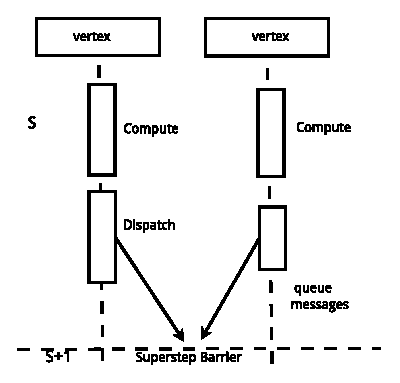
\includegraphics[width=\textwidth]{myfigures/sequentialbsp_new}
\caption{传统BSP模型}\label{fig:traBSP}
\end{minipage}
\begin{minipage}{0.4\textwidth}
\centering
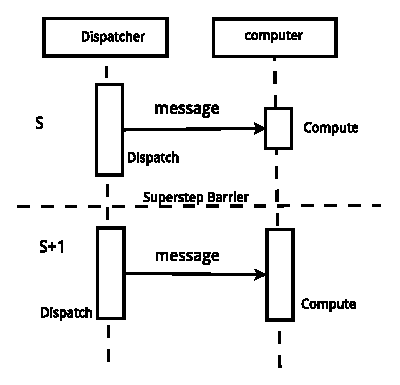
\includegraphics[width=\textwidth]{myfigures/computemodel}
\caption{改进后的BSP模型}\label{fig:newBSP}
\end{minipage}
\vspace{\baselineskip}
\end{figure}


\subsection{传统BSP模型的缺陷}
由于BSP模型的同步路障机制的存在,那么在整个BSP模型的垂直方向上,影响最终效率的关键就是最晚完成的任务,如图\ref{fig:bsp}所示。在基于传统BSP计算模型的图处理系统中,如图\ref{fig:traBSP}所示,图的处理主要分为两个阶段:以顶点为中心的计算(Compute)过程和消息的分发(Dispatch)过程。这两个过程按照严格的串行方式执行的,消息分发过程对计算过程存在数据依赖,形成强耦合。这种串行执行的方式,进一步延长了垂直方向上的任务完成的时间,降低的执行效率。在以顶点为中心的图计算中,消息时顶点之间的主要数据交换,顶点调用用户提供的计算函数对数据进行处理。消息包含计算所需的全部数据,所以相对于计算过程而言消息的具体分发过程是可以透明的。由于消息的生成和处理分布在两个相邻的超级步中,在该超级步结束之前,需要缓存大量的消息,并且在下一个超级步开始之前,这些消息不会被处理掉,增加额外的IO开销。
目前,基于BSP计算模型的图处理系统多任务并行处理的方法主要是采用多线程的技术。而线程是操作系统的基本调度单位,在操作系统中利用多线程在并发度上就会受到很大的限制。另外,由于需要保存大量的数据,当线程处理IO操作的时候,线程的调度会引发上下文的频繁切换,会对处理效率造成影响。

\subsection{Actor-BSP模型}

消息的分发过程和计算过程之间的主要依赖关系是消息,那么消息分发过程是消息的生产者,计算过程则是消息的消费者,两者之间以生产者和消费者的模式进行共存,从而将两者从严格串行的模式中解耦出来,如图\ref{fig:newBSP}所示。在改进后的BSP模型中,消息分发过程和计算过程位于两个单独的执行流程中。消息分发过程主要负责消息的生成和转发。计算过程侦听消息,当消息达到,计算过程则负责对消息进行处理及数据更新。
在语义上计算过程和消息分发过程是相互独立的轻量级调度单位。现有的BSP的实现在语义封装上往往是以顶点为中心,线程负责处理顶点。所以,在实现New BSP的模型中,采用轻量级、能够异步处理消息的并发模型成为关键。Actor并发模型相比于线程而言更加轻量级,有着更好的并发度。同时,Actor在语义上与Vertex的语义较为接近,兼顾了线程的调度执行和以顶点为中心的特点。

\subsection{Actor-BSP模型的优势}

Actor-BSP模型是在执行过程上完全异步计算的模型,计算过程与消息分发过程想分离,使得两个过程可以在一定程度上并行执行,充分利用多核的优势。

首先,在Actor-BSP模型中,Actor分为两种类型:负责消息分发过程的分发Actor和负责计算过程的计算Actor。得益于分发Actor和计算Actor之间的松耦合设计,两者之间的映射关系变得相当的灵活,缩短BSP模型在垂直方向上的执行流程,提高效率。

其次,分发Actor 和 计算Actor 组成了生产者和消费者模型,当消息到达计算Actor之后,该actor会被调度执行,处理消息,从而无需保存这些消息,避免将消息进行缓存的IO开销。

\section{数据组织}

单机的图处理系统同时具有计算密集型和IO密集型两个特点,合理的数据组织方式对整个系统的性能具有重要的影响。本节首先分析在Actor-BSP模型中数据的访问行为,然后根据数据的行为对GPSA的数据的组织方式进行说明和解释。

\subsection{数据访问行为}
在Actor-BSP模型中,Actor替换顶点成为整个计算展开的中心对象,之前顶点之间的消息的传递转变为Actor对象之间的消息通讯,从而导致新模型在数据读写方式上与传统的BSP模型不同。本小节从消息、顶点以及边的角度出发结合Actor-BSP模型展示其数据读写方式的行为特征。

首先,消息无需缓存。由于Actor-BSP模型中,由于生产者和消费者的组合,计算Actor监听消息到达事件,一旦事件到达消息就可以被及时处理。新模型无需为下一个超级步保存大量的消息,减少消息缓存的IO操作。

其次,只有分发Actor才会访问边。由于分发Actor主要任务就是生产消息,而消息的产生和发送都与边有着紧密的联系。但是,计算Actor不关心边的状态,只关心消息到达的事件以及如何处理消息与更新数据。

再次,顶点状态数据信息需要常驻内存来支持随机访问。在以顶点为中心的模型中,顶点是有状态信息的,当顶点开始对消息进行处理的时候,顶点自身的状态会包含在自己的数据域,并且参与到计算中。无状态的Actor不会持有特定消息所有者的顶点状态信息。如果计算Actor接收到消息,它需要获取消息所有者的状态信息,然后调用用户提供的函数对消息进行处理。然而无状态的Actor并不记录消息到来的顺序及消息所有者的任何信息,所以无状态的Actor在处理消息的时候需要能够随机获取消息所有者的状态信息。

最后,双份状态信息同时参与计算。在传统模型中,顶点的状态信息需要额外保存一份来判断状态是否发生更新。而在Actor-BSP模型中,顶点的状态信息的双份保存主要是因为分发Actor和计算Actor对状态信息读取的目的不同。分发Actor获取顶点的状态信息主要是产生消息,而计算Actor获取状态信息主要是用于处理消息,并且替换更新的状态信息。所以两者在获取的状态信息是不一致的。分发Actor获取的状态信息主要是来自初始化或者上一个超级步的结果,而计算Actor获取的状态信息却总是当前超步的最新结果。



\subsection{磁盘IO}
GraphChi和X-stream需要将大量的数据写入到磁盘中,因此对提高IO的性能有着非常高的要求。所以,Graphchi不遗余力的设计平行滑动窗口(PSW),并藉此实现异步的计算模型,并且为了实现PSW,GraphChi需要做非常多的预处理来满足要求。而X- stream也是从避免随机访问的角度出发采用顺序访问的Scatter和Gather两个阶段对图进行处理,同时采用异步IO的方式来获得更好的性能。

然而,在新的计算模型中,数据的访问方式发生较大的变化。不需要缓存消息意味着不需要为缓存大量的中间消息设计复杂的磁盘IO功能。边与顶点的分离,使得要处理的数据量减少很多。相比较整个庞大的图而言,顶点的状态信息就显得适合常驻内存进行处理来获取更好的性能。由于不需要向磁盘写入大量的数据,出于容错性的考虑,我们采用内存映射的方式对顶点的状态信息进行组织。而对于庞大数量的边而言,松散的组织结构可以省去一些耗时较长的预处理,同时满足顺序访问的特点,避免复杂的IO优化操作。

\subsection{数据组织设计}
图的数据主要分为两个部分,顶点的状态信息和边。其中,顶点的状态信息以二进制的格式存储在内存映射文件当中。边则以行压缩(Compressed Sparse Row)格式保存在磁盘上。

\begin{figure}[htbp]
\centering
\begin{minipage}{0.4\textwidth}
\centering
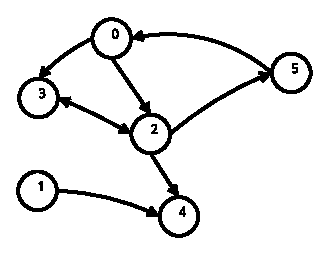
\includegraphics[width=\textwidth]{myfigures/graph.eps}
\caption{例图}\label{fig:graph}
\end{minipage}
\begin{minipage}{0.4\textwidth}
\centering
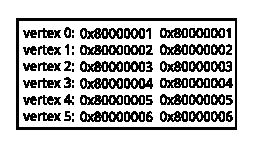
\includegraphics[width=0.8\textwidth]{myfigures/twocol.eps}
\caption{两列存储}\label{fig:twocol}
\end{minipage}
\begin{minipage}{0.4\textwidth}
\centering
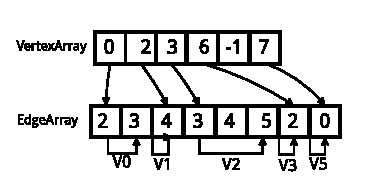
\includegraphics[width=\textwidth]{myfigures/csr.eps}
\caption{CSR存储}\label{fig:csr}
\end{minipage}
\begin{minipage}{0.4\textwidth}
\centering
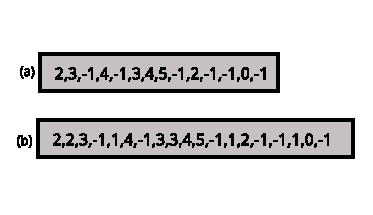
\includegraphics[width=\textwidth]{myfigures/ncsr.eps}
\caption{顺序存储}\label{fig:ncsr}
\end{minipage}

\vspace{\baselineskip}
\end{figure}

由于顶点的状态信息需要保存两份以供两种actor访问,所以在顶点状态信息的内存映射文件中,同一个顶点的状态信息以相邻的方式保存两份,就如同两排并列的数据,如图\ref{fig:twocol}所示。通过这种简单的方式,可以通过顶点\textit{id}计算顶点在整个文件中的偏移值来快速的获取顶点\textit{V}的状态信息的值,即$|V| * sizeof(Val)*2$。当该内存映射文件被映射到内存中后,整个访问的过程就像在操作一个数组一样方便。

CSR格式将顶点\textit{id}和边分别用两个数组进行保存,其中边数组保存边的目的顶点\textit{id}并按照出发顶点\textit{id}排序就,而在顶点数组中顶点的\textit{id}就是数组的索引,每个顶点保存第一条边在在边数组中的索引。此时,如果需要遍历第\textit{i}个顶点的边,那么只需要访问EdgeArray[VertexArray[i]],EdgeArray[VertexArray[i]+1],···,EdgeArray[VertexArray[i+1]]就可以完成该顶点边的遍历。如图\ref{fig:csr}所示,在遍历顶点\textit{Vertex 2}时,就可以通过访问[EdgeArray[3],EdgeArray[6])对边顶点进行遍历。CSR格式的空间效率是O(n+m),其中n和m分别是边和顶点的个数。另外,还可以在CSR格式的基础上采用顺序存储的方式,每个不同顶点的边之间用分割符加以分别,如图\ref{fig:ncsr}(a)所示,不同顶点之间可以用\textit{-1}作为分隔符,对边的遍历只需要读取到-1为止即可,除此之外还可以保存除边之外的其他信息,例如出度,权值等,在图\ref{fig:ncsr}(b)中就额外保存了每个顶点的出度,数组中第一个索引位置的值是2,表示此处顶点的的出度是2,紧接着的是两条边,当读取到-1的时候,顶点的\textit{id}递增加一。

\section{消息分发}
消息是本系统的重要关注和处理的对象,虽然Actor-BSP模型的优势使得无需为消息进行额外的缓存,但是合理的消息产生和分发策略对系统的效率有着重要的影响。
\subsection{消息}
一般来说消息的主要有两部分内容组成:目的顶点和消息的值。目的顶点表明该消息前往的顶点,同时也会影响由哪个具体的计算Actor来处理该消息。消息的值则是计算Actor用来进行计算的数据。虽然消息的生成工作主要是由分发Actor负责,但是消息的值的生成方法根据应用的不同具体的生成算法也不一样。例如,在遍历应用中,消息的值则是一个表示从源点开始到目前顶点的一个层次数,而在PageRank算法中,消息的值则是当前顶点的权值均分到他的出边邻接顶点的浮点数。所以,具体的消息的实现过程,由用户自己实现,分发Actor则调用具体的生成算法产生消息。
\subsection{分发策略}
当消息生成之后,分发Actor需要将消息分发给计算Actor。在Actor-BSP模型中,以顶点为中心的方式被无状态的Actor代替,计算Actor需要均衡的处理这些消息。虽然Actor的上下文切换远比线程轻量级,但是Actor的调度依然可能成为性能的制约因素,所以需要对消息的分发过程进行额外的硬性控制来避免某个计算Actor的负载过重。理论上来说,每个计算Actor都应该处理差不多个数的消息,但是由于图结构是无规律的,消息的发送目的地也有很大程度的随意性,在短时间内平均的将消息发送给计算Actor的可能性也微乎其微。为达到这样的目的,GPSA在预处理阶段对计算Actor进行了任务分配,将消息按照目的顶点的次序均分给计算Actor。在分发的过程中,如果某个计算Actor的邮箱已满,无法接受更多消息,那么该消息将会发送到目前消息数目最少的计算Actor的邮箱中,从而实现动态均衡。

\section{数据更新}
计算Actor接收到消息之后,调用用户实现的具体计算函数,如果经过计算之后顶点的状态发生改变,那么计算Actor就需要更新顶点的状态信息写入内存。由于计算Actor和分发Actor对数据访问的行为不同,所以需要两份不同的顶点信息的拷贝。其中一份拷贝供分发Actor查询使用,该数据是上一个超级步后的结果;另外一份拷贝则供计算Actor进行更新。由于两份数据以“Two-Column”的方式进行保存,两份数据就可以以列进行区分,如图\ref{fig:vu}所示。计算Actor和分发Actor对这两列数据依次交替访问,计算Actor访问的数据列是计算列,而分发Actor访问的数据列是分发列。

\begin{figure}[htbp]
\centering
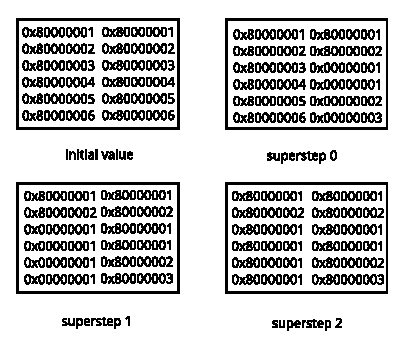
\includegraphics[width=0.4\textwidth]{myfigures/valueupdating.eps}
\caption{数据更新}\label{fig:vu}
\vspace{\baselineskip}
\end{figure}

在初始化结束之后,顶点的两列状态信息是相同的。分发Actor访问分发列的数据,然后计算Actor对计算列数据进行更新。在计算的过程中,为了避免消息的重复发送,同时保证计算Actor能够取得正确的顶点状态数据,将状态数据的最高位作为标识位。如果高位为1并且超级步\textit{i}大于0,则表示该数据在上一个超步中没有发生更新,分发Actor将会跳过该顶点,若高位为0,则说明数据在上一个超级步发生了更新,分发Actor会将此处数据对应的顶点的更新消息发送给它的邻接顶点,然后分发Actor将其高位置0。若超级步为0,则分发Actor会依次将顶点的状态信息发送出去。对于计算Actor,如果读取到的数据高位为1,则表明该数据尚未被更新,此时计算Actor将会读取该顶点的最新的状态信息,即从分发列对应位置获得最新值,如果计算之后顶点状态信息发生更新则把计算之后的新数据写入到当前顶点的计算列,否则不更新,下次读取数据依然从分发列读取数据。若计算Actor读取到的数据高位为0,则表明当前位置的数据是最新的,将会直接读取数据进行计算。如图\ref{fig:vu}所示,在初始化时,两列数据都相同并且最高位都为0。在超级步\textit{0}中,分发Actor对所有顶点的状态信息发送出去,计算Actor在接收到消息之后对计算列的数据进行更新。在超级步\textit{1}中,计算列和分发列互换位置,根据高位信息依次进行消息分发和数据更新。

\section{GPSA实现}
% 在上文,我们详细的分析了GPSA的设计细节,本部分则对GPSA的功能模块和实现过程进行详细的阐述。
% 在Actor-BSP模型的基础上,本文提出了基于新模型的单机图处理系统GPSA。通过实验证明,GPSA是一个具有高效、可扩展性与容错性的单机图处理系统。GPSA主要用JAVA编程语言实现,其中角色模型的实现采用了Kilim并发框架。本节将会对GPSA的组成和实现的过程进行详细的阐述。

GPSA的实现基于JAVA和Kilim角色并发框架。在GPSA中,输入是在上文中详述的以二进制形式保存的数据文件,包括顶点的状态信息和边的信息;输出则是经过计算之后图中顶点的状态信息。如图\ref{fig:overview},GPSA主要包括三个功能模块:预处理、Manager管理模块、Actor工作模块。预处理模块主要涉及对计算开始之前的初始化工作;Manager管理模块负责对计算进行协调与控制;分发Actor负责消息的产生和分发;计算Actor则是计算的基本执行单元。

·
\begin{figure}[htbp]
\centering
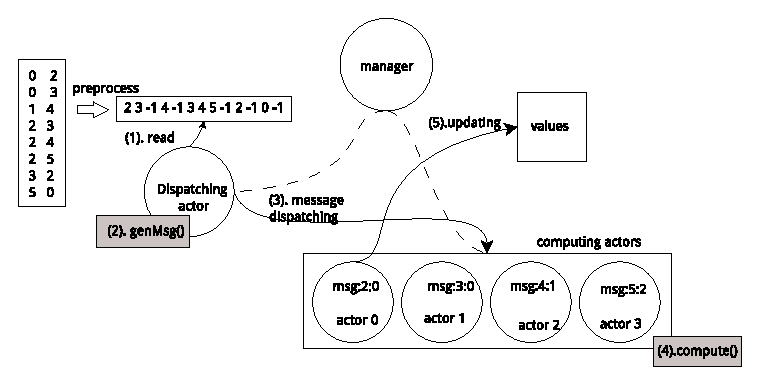
\includegraphics[width=0.8\textwidth]{myfigures/newexample.eps}
\caption{系统架构}\label{fig:overview}
\vspace{\baselineskip}
\end{figure}

\subsection{预处理}
GPSA默认对边集存储的数据进行预处理。
首先,边按照起始顶点的大小升序排序。虽然GPSA的新模型对分发过程和计算过程进行了分离,GPSA理论上只要能够获取边、起始顶点的顶点状态信息和用户自定义的消息生成的函数就可以发送消息并驱动计算Actor进行计算,也就是说GPSA可以处理原始的以边集存储的图。但是GPSA的新模型仍然是基于BSP模型的,耗费时间最长的任务将决定实际的计算效率,而直接对原始的边集数据进行计算,容易造成任务分配不均,计算效率低的结果。另外,在新模型中图的顶点信息是需要进行初始化并且映射到内存中的,需要与边区别对待。
在GPSA中,图是以CSR的格式进行存储的,需要将顶点和边分开,计算出图的一些基本信息,例如,边数、顶点数等,同时对任务进行分割。首先,预处理模块读取边,对边按照起始顶点的大小按升序的方式进行排序,如果起始顶点相同则按照目的顶点的大小升序排序。接下来,对排序之后的边进行CSR格式转换,将转换后的CSR格式的图数据写入磁盘,同时计算出图的基本信息,例如顶点的出度和入度、顶点个数,边的个数等等。

任务分割主要指计算任务的分割。对于消息分发Actor而言,顺序读取CSR数据即可;对于计算Actor而言,每个计算Actor所处理的消息个数应该相差不大,同时为避免有两个Actor同时操作同一顶点信息的更新而引起同步写,所以GPSA采用了一种“区间”的处理方法,即每个计算Actor负责连续的顶点闭区间$[i,j]$,每个区间接受的消息总数目接近每个计算Actor负责消息的平均值。

假设图的总边数为\textit{m},计算Actor个数为\textit{n},则每个计算Actor的区间处理的消息数目为\textit{k}满足以下条件:

\[\frac{m}{n} \le k < \frac{m}{{n - 1}}\]

预处理模块根据顶点的入度计算每个Actor所应处理的消息个数,并生成响应的区间对象,将其传递给Manager管理者。
\subsection{Manager管理模块}
Manager主要负责初始化计算,协调分发和计算的有序进行以及异常处理。在计算开始执行之前,图数据需要准备就绪,Manager调用预处理模块对图进行处理,根据图的基本信息计算出最小的顶点\textit{id}和最大的顶点\textit{id},调用用户定义初始化函数对顶点的状态信息进行初始化,并将结果写入顶点信息内存映射文件,完成对顶点初始信息的初始化。另外,manager需要根据用户指定的分发Actor和计算Actor数目,初始化对应数目的Actor。

初始化工作完成之后,Manager主要对计算过程进行协调。如算法\ref{algo:manager}所示,首先Manager向分发Actor发送\textit{ITERATION\_START}信号。接收到\textit{ITERATION\_START}信号的分发Actor会开始访问存储在磁盘上的CSR格式的图数据,调用用户定义的消息生成规则函数打包消息。当分发Actor在当前超级步的消息分发任务完成之后,分发Actor用\textit{DISPATCH\_OVER}信号通知Manager。如果所有的分发Actor都完成之后,Manager紧接着向所有的计算Actor发送\textit{COMPUTE\_OVER}信号。如果计算Actor处理到该消息则会意识到本超级步的计算工作已经完成,此时它会回复Manager一个同样的\textit{COMPUTE\_OVER}。最后,如果计算满足结束条件,Manager向所有的Actor发送\textit{SYSTEM\_OVER},当Actor接受到该信号将会退出自身的执行循环,结束生命周期。

\begin{algorithm}[htb!]
{
{

\renewcommand\baselinestretch{1.5}\selectfont %控制行距

\caption{Manager Execution Loop}
\label{algo:manager}
\begin{algorithmic}[1]
\REQUIRE ~\\
Initialize dispatchers,computers,mailbox, 

\STATE $counter \leftarrow 0$
\STATE $currIte \leftarrow 0$

\WHILE{ $currIte < endIte$ }
\FOR {$dispatcher \in dispatchers$}
\STATE $dispatcher \leftarrow ITERATION\_START$
\ENDFOR

\WHILE{ $(signal \leftarrow mailbox.get()) == DISPATCH\_OVER$}
\STATE $counter \leftarrow counter + 1$
\IF{$counter == dispatchers.length$}
\STATE $counter \leftarrow 0$
\STATE $break$
\ENDIF
\ENDWHILE

\FOR {$worker \in computers$}
\STATE $worker \leftarrow COMPUTE\_OVER$
\ENDFOR

\WHILE{ $(signal \leftarrow mailbox.get()) == COMPUTE\_OVER$}
\STATE $counter \leftarrow counter + 1$
\IF{$counter == computers.length$}
\STATE $counter \leftarrow 0$
\STATE $break$
\ENDIF
\ENDWHILE

\STATE $currIte \leftarrow currIte + 1$
\ENDWHILE
\end{algorithmic}
}
\par}
\end{algorithm}

\subsection{Actor工作模块}
Actor模块系统中最重要的组成部分,该模块主要负责消息的生成和计算并更新数据。在该模块中主要包含两种无状态Actor:分发Actor和计算Actor。

%分发Actor从磁盘上顺序读取边,根据初始化信息或者上个超级步中顶点的更新情况,调用用户自定义的消息产生函数生成新消息,并将消息发送到边的目的顶点所对应的计算Actor。
分发Actor的工作流程如算法\ref{algo:dispatcher} 所示,分发Actor等待来自Manager的\textit{ITERATION\_START}的信号,接收到信号后分发Actor开始进入执行循环,检查处理的边的起止信息,从起止信息的起始位置开始顺序从磁盘上读取一条边,获取该边起始顶点的顶点的状态信息,如果当前超级步不是0并且信息高位为1,则表明当前顶点的状态信息在上一个超级步中没有发生更新,需要跳过该顶点,继续处理下一个顶点,\textit{skip(sequence)}函数,则会让当前的的顶点\textit{id}加1,同时跳过该顶点的所有边,寻址到下一个顶点的第一条边的偏移地址。若当前超级步为0或者高位为0,则表明该顶点处于初始化之后的状态或者在上一个超级步中发生了更新,分发Actor调用用户提供的\textit{genMsg()}实现生成消息,根据分发策略将消息发送出去。如果读取边的目的顶点为-1,则表明当前顶点处理完毕,并将该顶点的状态信息状态最高位置1表明处理完成。如此周而复始,直至完成分发任务,分发Actor用\textit{DISPATCH\_OVER}通知Manager。

\begin{algorithm}
{
{

\renewcommand\baselinestretch{1.5}\selectfont %控制行距

\caption{Dispatcher Execution Loop}
\label{algo:dispatcher}
\begin{algorithmic}[1]

\STATE
 $signal \leftarrow mailbox.get()$
\WHILE{ $signal != SYSTEM\_OVER$ }
\IF{$interval != null$}
\STATE $ reset() $
\WHILE{$curoff < endoff$}
\STATE $val \leftarrow getValue(sequence)$

\IF{$isHighestBit(val)==1 \&\& currIte != 0$}
\STATE $skip(sequence)$
\ENDIF

\IF{$isHighestBit(val)==0 \|\| currIte == 0$}
\STATE $vid \leftarrow readEdge(curoff)$
\WHILE{$curoff < enfoff $}
\IF{$vid == -1$}
\STATE $break$
\ENDIF
\STATE $msg \leftarrow genMsg()$
\STATE $DispatchStrategy(vid,msg)$
\ENDWHILE
\STATE $setHighesetBitTo1()$
\ENDIF
\ENDWHILE
\ENDIF
\STATE $notifyManager(DISPATCH\_OVER)$
\STATE $signal \leftarrow mailbox.get()$
\ENDWHILE

\end{algorithmic}
}
\par}
\end{algorithm}


计算Actor的工作流程如算法\ref{algo:computer}所示,计算Actor等待来自Manager的消息,然后进入执行循环体。否则计算Actor从消息中提取目的顶点和消息的值,根据目的顶点从顶点的状态信息内存映射文件中读取顶点值,然后调用用户提供的\textit{compute(val,msgVal)}实现对其进行计算,计算返回一个新的顶点状态信息。如果新的顶点状态与之前的值相比发生了改变,则将新数据更新到内存映射文件,否则丢弃。如此迭代,直到计算Actor接受到的信号是\textit{COMPUTE\_OVER},则表示当前的超级步的计算完成,同时用\textit{COMPUTE\_OVER}回复Manager。如果计算Actor接收到\textit{SYSTEM\_OVER}信号,则会结束计算退出循环。

\begin{algorithm}
{
{
\renewcommand\baselinestretch{1.5}\selectfont %控制行距

\caption{Compute Execution Loop}
\label{algo:computer}
\begin{algorithmic}[1]

\STATE $msg \leftarrow mailbox.get()$
\WHILE{ $signal != SYSTEM\_OVER$ }
\IF{$msg == COMPUTE\_OVER$}
\STATE $notifyManager(COMPUTE\_OVER)$
\ELSE
\STATE $to \leftarrow msg.dest()$
\STATE $msgVal \leftarrow msg.val()$
\STATE $val \leftarrow getVal(to)$
\STATE $newVal \leftarrow compute(val,msgVal)$
\IF{$newVal != val$}
	\STATE $update()$
\ENDIF
\ENDIF
\STATE $msg \leftarrow mailbox.get()$
\ENDWHILE


\end{algorithmic}
}
\par}
\end{algorithm}


\section{小结}

本章首先介绍常见的用于图计算的模型,并讨论了BSP模型中的缺陷。接下来在传统BSP模型的基础上,使用Actor将计算过程和分发过程分开。然后围绕Actor-BSP模型中的数据行为、磁盘IO、消息分发和数据更新等内容对GPSA系统进行设计和规划。最后,在此基础上,本章对GPSA的系统实现进行阐述和说明。从功能模块上划分,GPSA主要分为预处理模块、Manger管理模块、计算Actor和分发Actor模块。预处理模块对数据进行数据格式的转换与信息分离,以及任务分配等工作。Manager则是系统的执行计算的控制单元,负责协调计算Actor和分发Actor的开始和进行,以及一些异常处理。计算Actor和分发Actor模块则是主要的运算模块,其中分发Actor从磁盘读取一条边,根据用户的消息生成规则产生消息,并将消息分发给计算Actor,而计算Actor在接受到消息之后,会根据消息访问顶点信息,调用用户的\textit{compute(val,msgVal)}函数进行计算并取得返回值,然后判定是否发生更新,并将更新数据写入内存。
